\section{Learning to Memorize at Test Time}\label{sec:mem-module}
\lettrine[lines=3]{T}{}o overcome the lack of long-term memory and to enable the model to learn, forget, and retrieve information, in this section, we present a neural long-term memory module, which is a meta models that learns to memorize at test time. In \autoref{sec:long-memory}, we first discuss the motivation and the design of the neural memory.  In \autoref{sec:fast-training}, we discuss how our architecture design can benefit from a fast and parallelizable training. Finally, in \autoref{sec:persistent-memory}, we augment our architecture using persistent memory module, in which we use learnable but data-independent parameters to learn meta information about the task. 




\subsection{Long-term Memory}\label{sec:long-memory}
To design a neural long-term memory module, we need a model that can encode the abstraction of the past history into its parameters. An example of this can be LLMs that are shown to be memorizing their training data~\citep{staab2024beyond, schwarzschild2024rethinking, leybzon2024learning}. Therefore, a simple idea is to train a neural network and expect it to memorize its training data. Memorization, however, has almost always been known as an undesirable phenomena in neural networks as it limits the model generalization~\citep{bayat2024pitfalls}, causes privacy concerns~\citep{staab2024beyond}, and so results in poor performance at test time. Moreover, the memorization of the training data might not be helpful at test time, in which the data might be out-of-distribution. We argue that, we need an online meta-model that learns how to memorize/forget the data at test time. In this setup, the model is learning a function that is capable of memorization, but it is not overfitting to the training data, resulting in a better generalization at test time.    

\head{Learning Process and Surprise Metric}
The key idea to train a long-term memory is to treat its training as an online learning problem, in which we aim to compress the past information $x_1, \dots, x_{t-1}$ into the parameters of our long-term neural memory module $\mathcal{M}_t$. As discussed earlier, an event that violates the expectations (i.e., is surprising) is more memorable for humans~\citep{mandler2014structure}. Inspired by this, a simple definition of surprise for a model can be its gradient with respect to the input. The larger the gradient is, the more different the input data is from the past data. Accordingly, using this surprise score, we can update the memory as:
\begin{align}\label{eq:GD}
    \M_{t} = \M_{t-1} - \theta_t \: \undermath{\text{Surprise}}{\textcolor{c4}{\nabla \ell(\M_{t-1}; x_{t})}}.
\end{align}
This surprise metric, however, can result in missing important information that comes after a big surprising moment. That is, the gradient can become extremely small after several surprising steps, leading to stocking in a flat area (i.e., local minima), and missing information about some parts of the sequence. From the human memory perspective, an event might not consistently surprise us through a long-period of time although it is memorable. The reason is that the initial moment is surprising enough to get our attention through a long time frame, leading to memorizing the entire time frame. To improve the above surprise metric (\autoref{eq:GD}), we break the surprise metric into (1) \emph{past surprise}, which measures the surprise amount of a very recent past; and (2) \emph{momentary surprise}, which measures the surprise of incoming data: 
\begin{align}\label{eq:GD-momentum}
    & \M_{t} = \M_{t-1} + \textcolor{c4}{S_{t}},\\
    & S_{t} = \eta_t \undermath{\text{Past Surprise}}{\textcolor{c4}{S_{t-1}}} - \theta_t\:  \undermath{\text{Momentary Surprise}}{\textcolor{c4}{\nabla \ell\left(M_{t-1}; x_{t} \right)}}.
\end{align}
Interestingly, this formulation is similar to gradient descent with momentum, where $S_{t}$ is the momentum element. Therefore, the momentum here act as a memory of surprise across time (sequence length). In this formulation, the term $\eta_t$ is a data-dependent surprise decay (a function of $x_t$), controlling how surprise decays over time, and the term $\theta_t$ is controlling how much of momentary surprise should be incorporated into the final surprise metric in a data-dependent manner. This data-dependency is particularly important in this design: While surprise of previous tokens might be needed to affect the surprise of the next token, it is mostly valid if all tokens are relevant and are in the same context. Accordingly, a data-dependent $\eta$ can control if memory needs to: (1) ignore the last surprise by setting $\eta_t \rightarrow 0$ (possibly due to the change of context), or (2) fully incorporate the last surprise by setting $\eta_t \rightarrow 1$ (possibly as the token is highly relevant to its recent past tokens). 







\head{Objective}
Our above surprise metric is based on a loss function $\ell(.;.)$, which is the objective that our memory is learning to act as it at test time. That is, our memory module is a meta model that learns a function based on the loss function $\ell(.;.)$. In this work, we focus on \emph{associative memory}, in which we aim to store the past data as the pairs of keys and values. Given $x_t$, similar to Transformers~\citep{transformers}, we use two linear layers to project $x_t$ into a key and value:
\begin{align}
    \mathbf{k}_t = x_t W_K, \qquad \qquad  \mathbf{v}_t = x_t W_V,
\end{align}
where $ W_K$ and $W_V \in \R^{d_{\text{in}} \times d_{\text{in}}}$. Next, we expect our memory module to learn the associations between keys and values. To this end, we define the loss as follows:
\begin{align}\label{eq:loss}
    \ell(\M_{t-1}; x_t) =\left \Vert \M_{t-1}\left(\mathbf{k}_t\right) - \mathbf{v}_t  \right \Vert_2^2  
\end{align}
By optimizing the above loss function in the inner-loop of our meta model (memory), the model learns how to memorize the mapping between keys and values at test time. Note that, similar to meta-learning models~\citep{zintgraf2019fast, nichol2018first}, training of the memory is in the inner-loop, and so parameters $W_K$ and $W_V$ are hyperparameters in the above loss function. Accordingly, in the inner loop, we optimize $\M$'s weights, while in the outer-loop, we optimize other parameters of the entire architecture. 

\head{Forgetting Mechanism}
When dealing with very large sequences (e.g., millions of tokens), it is crucial to manage which past information should be forgotten–even with a deep or a very large matrix-valued memory. To this end, we use an adaptive forgetting mechanism that allows the memory to forget the information that is not needed anymore, resulting in better managing the memory's limited capacity. That is, given the next token $x_t$, we modify the update rule as:
\begin{align}\label{eq:all}
    & \M_{t} = (1 - \alpha_t) \M_{t-1} + \textcolor{c4}{S_{t}},\\
    & S_{t} = \eta_t {\textcolor{c4}{S_{t-1}}} - \theta_t\:  {\textcolor{c4}{\nabla \ell\left(M_{t-1}; x_{t} \right)}},
\end{align}
where $\alpha_t \in [0, 1]$ is the gating mechanism that flexibly controls the memory; i.e., decides how much information should be forgotten. For example, it can update the memory without affecting the past abstraction by letting $\alpha_t \rightarrow 0$, and can clear the entire memory by letting $\alpha_t \rightarrow 1$. Later in this section, we show that this weight decay mechanism is closely related to the gating mechanism in modern RNNs~\citep{dao2024transformers, orvieto2023resurrecting}. 


\head{Memory Architecture} 
In this paper, we focus on simple MLPs with $L_{\M} \geq 1$ layers as the architecture of our long-term memory. The main reason behind this choice is that we want to focus on better motivating the design of the long-term memory and ways that it can be incorporated into an architecture.  However, our formulation and architectural design opens a new research direction to design neural architectures that are more effective and efficient in memorization of data. Recently, there has been a promising line of work to design such architectures~\citep{zhang2024memory, cetin2024evolved, berges2024memory}, which incorporating them into our framework (i.e., replacing simple MLPs with such architectures) can be an interesting future work. 


When using vector-valued or matrix-valued memory~\citep{yang2024gatedattn, orvieto2023resurrecting, de2024griffin}, the memory module is compressing the past data and fit it into a line. That is, from the meta learning or online learning perspective~\citep{sun2024learning}, using a matrix-valued memory $\M = W \in \R^{d_{\text{in}} \times d_{\text{in}}}$ is equivalent to optimize $\ell(W_{t-1}; x_t) =\left \Vert W_{t-1}\mathbf{k}_t - \mathbf{v}_t  \right \Vert_2^2$, which is an online linear regression objective and so the optimal solution assumes the underlying dependency of historical data is linear. On the other hand, we argue that deep memory modules (i.e., $L_{\M} \geq 2$) . Aligning with the theoretical results that MLPs with at least two layers are strictly more expressive than linear models~\citep{hornik1989multilayer}, in \autoref{sec:deep-memory-exp}, we show that deep memory modules are more effective in practice.       





\head{Retrieving a Memory}
In the above, we discuss how one can design and train a long-term memory module that learns to memorize at test time. A key remaining question is: \emph{How one can retrieve information from the memory?} We simply use the forward pass without weight update (i.e., inference) to retrieve a memory correspond to a query. Formally, given an input $x_t$, we use a linear layer $W_{Q}$ to project the input, i.e., $\mathbf{q}_t = x_t W_{Q}$ and retrieve the corresponding (or useful) information from the memory ${y}_t$ by:
\begin{align}
    y_t = \M^*(\mathbf{q}_t).
\end{align}




\begin{figure*}
    \centering
    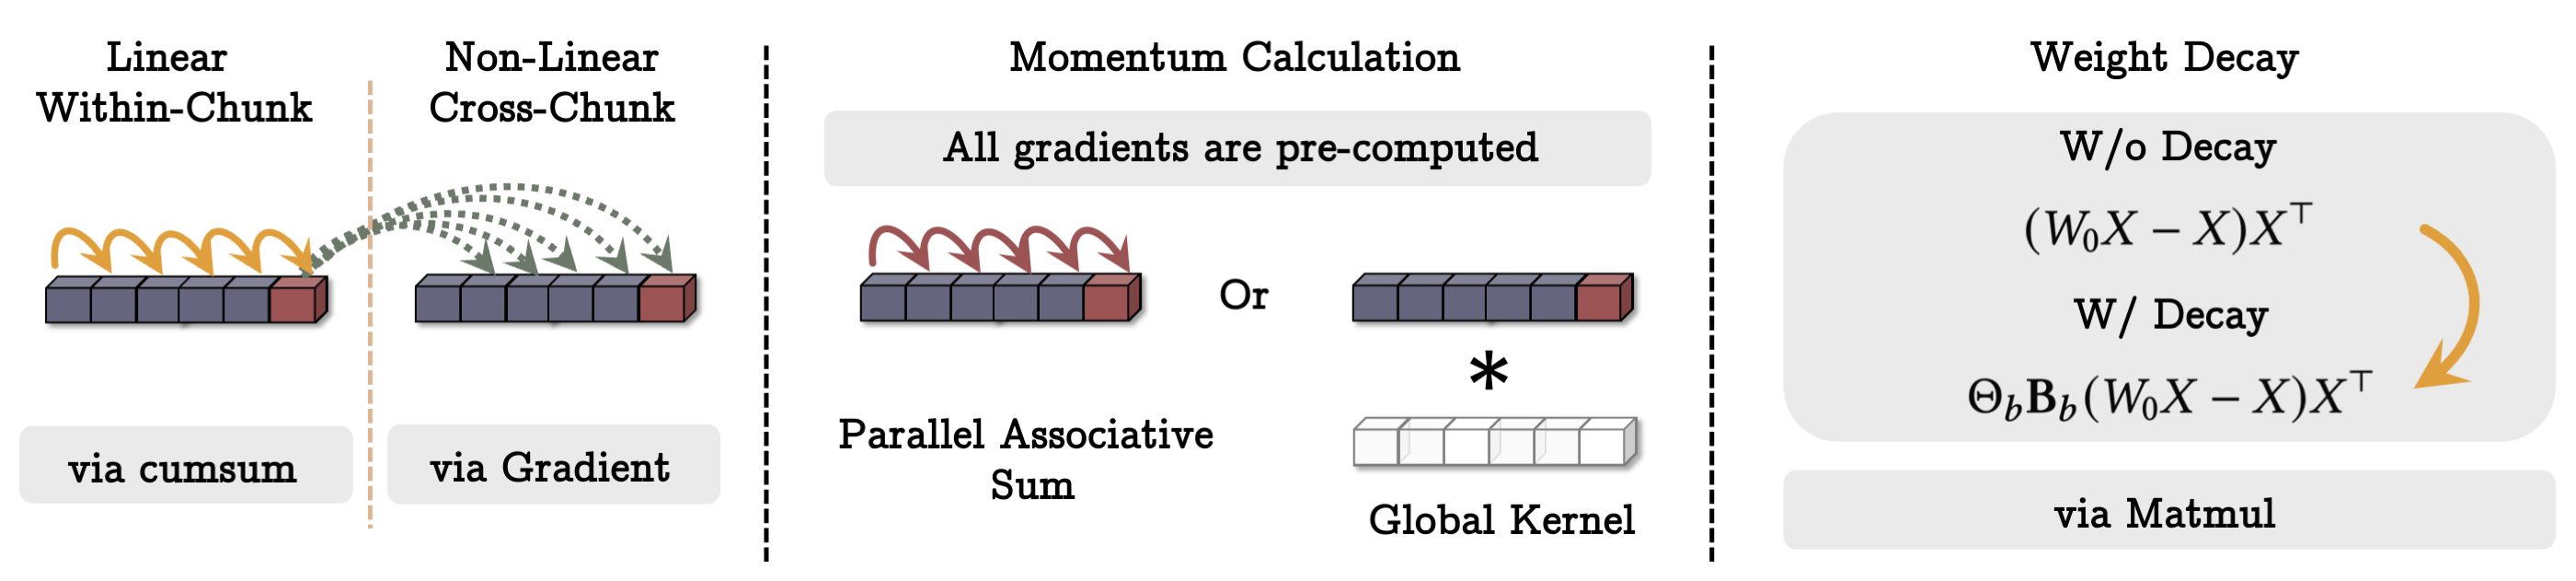
\includegraphics[width=0.8\linewidth]{Figures/Parallelization.png}
    \caption{The illustration of how the training of neural memory can be done in parallel and using \texttt{matmul}s.}
    \label{fig:parallel}
\end{figure*}

\subsection{How to Parallelize the Long-term Memory Training}\label{sec:fast-training} 
As discussed above, the design of our long-term memory module is equivalent to training a meta model by optimizing associative memory loss function $\ell(\M_{t-1}; x_t) =\left \Vert \M_{t-1}\left(\mathbf{k}_t\right) - \mathbf{v}_t  \right \Vert_2^2$ using gradient descent with momentum and weight decay. Therefore, in theory, the training of long-term memory module requires $\mathcal{O}\left(N\right)$ FLOPs, where $N$ is the sequence length. However, in practice, we need to parallelize the training process and to fully take advantage of hardware accelerators (e.g., TPUs, GPUs), we need to tensorize the process and use more \texttt{matmul}s. 

Next, we show that calculating the weights in the inner loop with mini-batch gradient descent, data-dependent learning rate, and weight decay can be reformulated so that it uses only \texttt{matmul}s and sum. We build upon the work of \citet{sun2024learning} that shows forward pass of a model optimizing with the mini-batch gradient descent (with constant learning rate) can be calculated using \texttt{matmul}s. We can split the sequence into chunks of size $b \geq 1$, and write the mini-batch gradient descent as:
\begin{align}
    \M_{t} = (1 - \alpha_t) \M_{t-1} - \theta_t \nabla \ell(\M_{t-1}; x_t) = \beta_{t} \M_0 - \sum_{i = 1}^{t} \theta_i \frac{\beta_{t}}{\beta_{i}} \nabla \ell(\M_{t'}; x_i),
\end{align}
where $t' = t - \texttt{mod}(t, b)$, and $\beta_{i} = \prod_{j=1}^{i}(1-\alpha_j)$. For the sake of simplicity, we focus on the first chunk, i.e., $t = b$ and so $t' = 0$. Also, we explain the process for the case that $\M_{t} = W_t$ is linear. The process for MLPs with $N_p \geq 2$ is similar. Using our loss function, we have:
\begin{align}\label{eq:weight-decay-matmul}
    \nabla \ell(W_{0}; x_t) =  (W_0 x_t - x_t) x_t^{\top} \Rightarrow \sum_{i = 1}^{b} \theta_i \frac{\beta_{b}}{\beta_{i}} \nabla \ell(W_{0}; x_i) = \Theta_b \mathbf{B}_b (W_0 X - X) X^{\top}, 
\end{align}
where $\Theta_b = \texttt{diag}\left(\begin{bmatrix}
    \theta_1 & \theta_2 & \dots & \theta_b
\end{bmatrix} \right)$ and $\mathbf{B}_b$ is defined analogously on $\frac{\beta_{b}}{\beta_{i}}$s. Note that, we do not need to store all $\Theta_{kb}$ and $\mathbf{B}_{kb}$ for $k = 1, \dots, N/b$, instead, we store these matrices for each chunk, resulting in using less memory. Next, we extend this representation so we can also incorporate the momentum term. In a chunk wise gradient descent with momentum, if we look at the momentum term, we have:
\begin{align}\label{eq:momentum-ssm}
    S_{t} = \eta_t {S_{t-1}} - \theta_t\:  u_t,
\end{align}
where $u_t = \nabla \ell\left(M_{t'}; x_{t} \right)$. Note that, we can compute all $u_t$ at the same time, and so \autoref{eq:momentum-ssm} is a linear recurrence with $u_t$ as an input, $S_t$ as the hidden state, and $\eta_t$ as input-dependent transition value. Accordingly, we can use parallel associative scan~\citep{smith2023simplified} to calculate $S_t$s in this chunk.  


\head{Parameters as the Function of Chunks}
Instead of making parameters like $\alpha_t, \theta_t$, and $\eta_t$ input-dependent (i.e., a function of token $x_t$), we can make them functions of their chunk. Despite losing expressive power, this formulation can help to make the training even faster. In this case, we are using the same value for each of $\alpha$, $\theta$, and $\eta$ in each chunk. Accordingly, in \autoref{eq:weight-decay-matmul}, we can store $\Theta$ using a single scaler. Similarly we can make \autoref{eq:momentum-ssm} faster. That is, when $\eta$ and $\theta$ are learnable but time-invariant inside each chunk, this equation becomes a linear time-invariant system (LTI), which can be computed by a global convolution~\citep{gu2022efficiently}. In our experiments, we make these parameters as the functions of tokens. However, such simplifications (i.e., as the function of chunks) can be the interest of future work to training larger models in more efficient manner.   




\subsection{Persistent Memory}\label{sec:persistent-memory}
Our long-term memory can also be seen as a contextual memory, meaning that the output is fully depend on the context. Therefore, in addition to our long-term memory, we also use a set of learnable but input-independent parameters to act as task-related memory. This type of memory has been referred to as persistent or meta-memory in the literature~\citep{sukhbaatar2019augmenting, dong2024hymba}. Given $N_p \geq 1$, we use learnable parameters $P = \begin{bmatrix}
    p_1 & p_2 & \dots & p_{N_p}
\end{bmatrix}$ and append it to the start of our sequence: i.e., given a context window size of $N$, we modify the input as:
\begin{align}
    x_{\text{new}} = \begin{bmatrix}
    p_1 & p_2 & \dots & p_{N_p}
\end{bmatrix} || \: \: x, 
\end{align}
where $||$ is concatenation. Next, we discuss the motivation of persistent memory from three perspective:




\head{Memory Perspective}
As discussed earlier, our neural long-term memory is a contextual memory, in which all parameters are input-dependent. An effective memory system, however, also needs input-independent parameters to store the abstraction of the task knowledge. That is, mastering a task requires the memorization of the knowledge that how the task can be done, and these parameters are responsible for storing such knowledge. 



\head{Feedforward Network Perspective}
In the Transformer architectures, there are fully connected layers after the attention module, which are shown to be similar to attention weights but with data-independent parameters. That is, \citet{sukhbaatar2019augmenting} showed that replacing the \texttt{ReLU} in fully connected layers with \texttt{Softmax} can results in an attention-like weights, in which weights are data-independent:
\begin{align}
    FFN(x) = W_V \: \texttt{Softmax}\left( W_K x\right).
\end{align}
In fact, $W_K$ and $W_V$ are acting similar to $K$ and $V$ matrices in attention module when they are input-independent. The persistent memory weights are expected to have the same functionality, meaning that using them in the first part of the sequence leads to having input-independent attention weights~\citep{sukhbaatar2019augmenting}. 


\head{Technical Perspective}
Attention with causal mask has implicit bias toward initial tokens in the sequence, and so attention weights are almost always highly active for initial tokens, resulting in performance damage. From the technical perspective, these learnable parameters at the start of the sequence can mitigate such effect by redistributing the attention weights more effectively~\citep{xiao2024efficient, hanLMInfinite2024}. 



\begin{figure*}[t!]
    \centering
    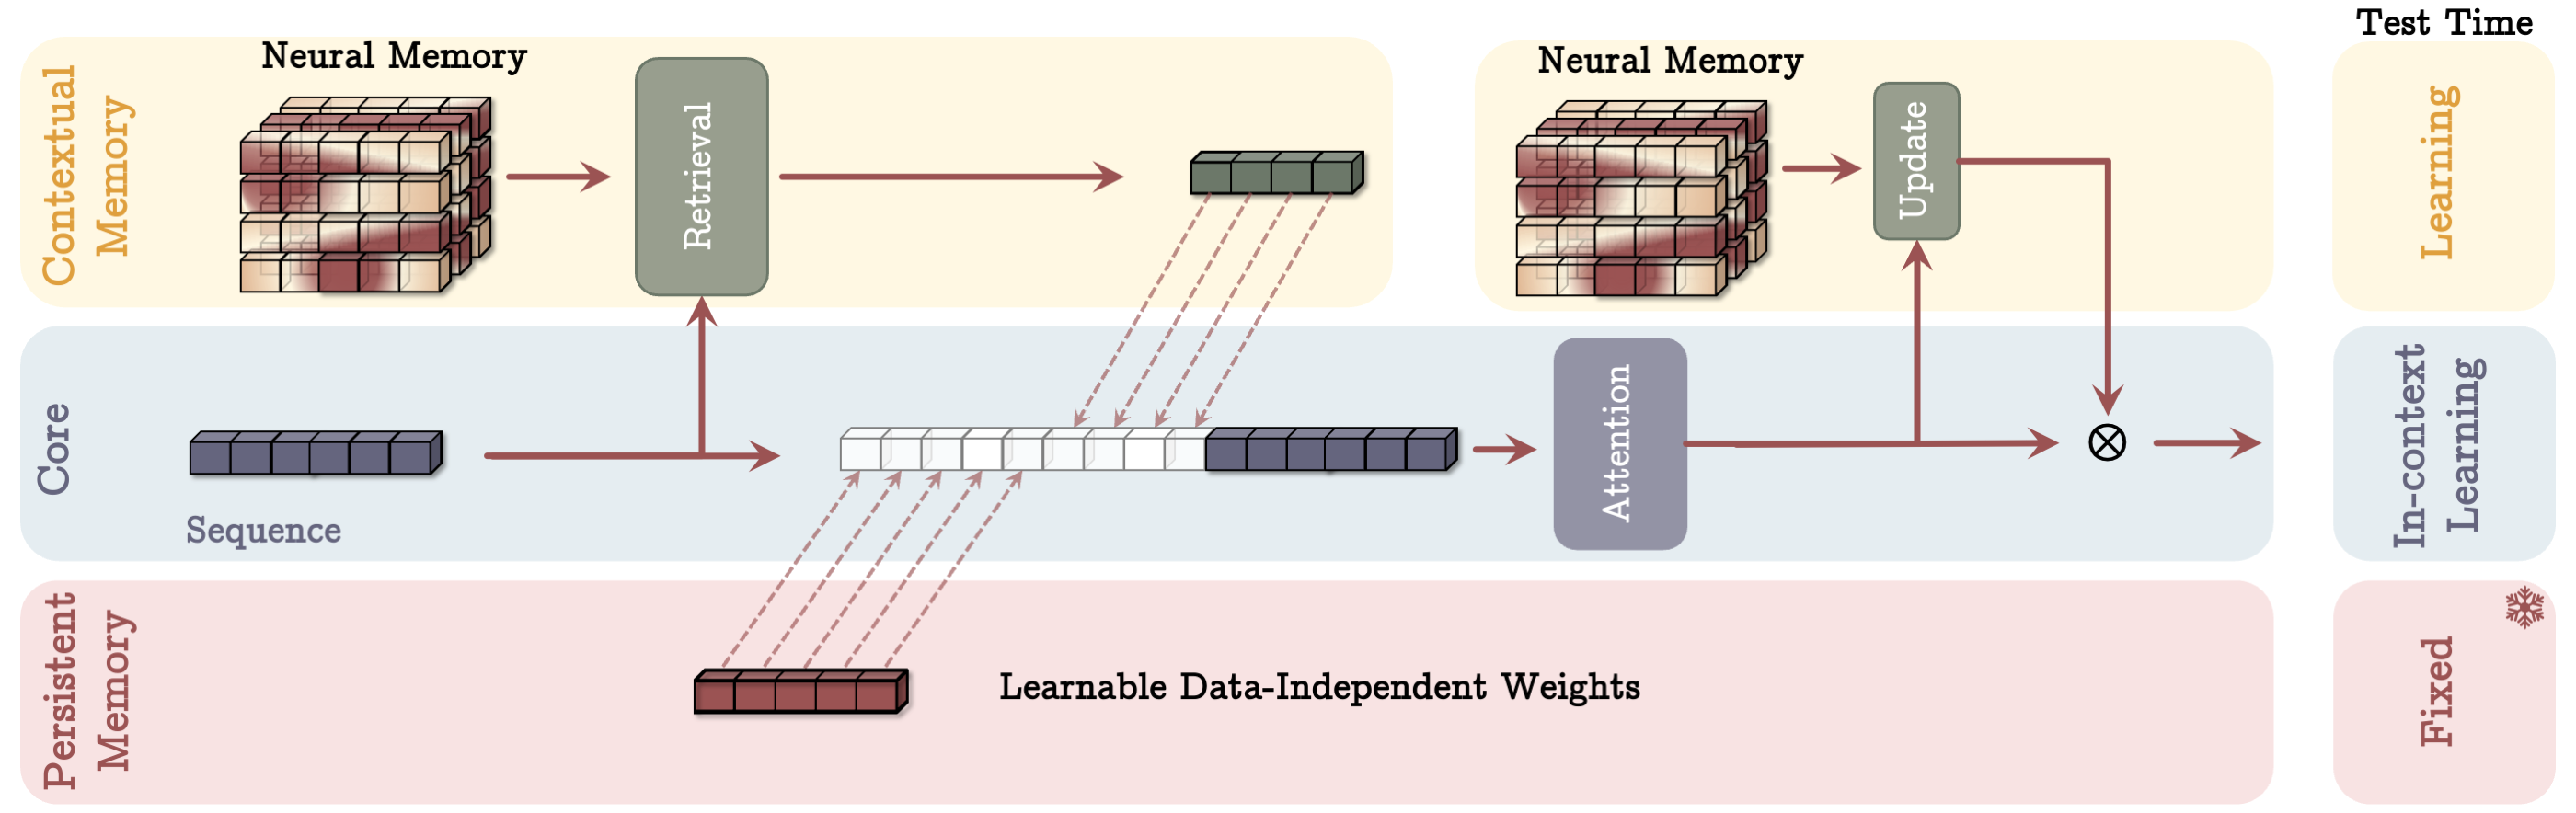
\includegraphics[width=0.9\linewidth]{Figures/loop-arch.png}
    \caption{\textbf{Memory as a Context (MAC) Architecture.} This architecture includes three branches of (1) core, (2) contextual (long-term) memory, and (3) persistent memory. The core branch concatenates the \emph{corresponding} long-term and persistent memories with the input sequence. Next, attention performs on the sequence and decides what part of the information should store in the long-term memory. At the test time, parameters corresponds to contextual memory are still learning, parameters corresponds to the core branch are responsible for in-context learning, and parameters of persistent memory are responsible to store the knowledge about tasks and so are fixed.}
    \label{fig:loop-arch}
\end{figure*}











\section{How to Incorporate Memory?}\label{sec:arch}
\lettrine[lines=3]{A}{}n important question that remained unanswered is: How one can effectively and efficiently incorporate the designed neural memory into a deep learning architecture? As discussed earlier, from a memory perspective, the pair of K and V matrices in transformers can be interpreted as an associative memory block. Due to their accurate modeling of dependencies and so their limited context window, we interpret them as short-term memory modules, attending to the \emph{current} context window size. On the other hand, our neural memory with the ability to continuously learn from data and store it in its weights can play the role of a a long-term memory. In this section, we aim to answer the above question by proposing three different variants of Titans. Later in our experiments, we show that each of these variants has its own advantages/disadvantages and also can show a trade-off between the efficiency and effectiveness in very long-contexts. 





\subsection{Memory as a Context}
In the first architecture design (see \autoref{fig:loop-arch}), we treat the memory as a context to the current information. That is, given a long sequence $x \in \R^{N \times d_{\text{in}}}$, we first chunk the sequence into fixed-size segments $\texttt{S}^{(i)}$ for $i = 1, \dots, N/C$. Given the incoming segment $\texttt{S}^{(t)}$, we consider it as the current context and its past segment as the historical information. Therefore, let $\M_{t-1}$ be the state of long-term memory before segment $\texttt{S}^{(t)}$, we use the input context as the query to the memory $\M_{t-1}$ to retrieve the corresponding information from the long-term memory. That is, we retrieve the past information that corresponds to $\texttt{S}^{(t)}$ as:
\begin{align}
    h_{t} = \M^{*}_{t-1} (\mathbf{q}_{t}),  
\end{align}
where $\mathbf{q}_{t} = \texttt{S}^{(t)} W_Q$. Next, we use this historical information along with our persistent memory parameters as the input sequence to the attention module:
\begin{align}
    &\tilde{\texttt{S}}^{(t)} = \begin{bmatrix}
    p_1 & p_2 & \dots & p_{N_p}
\end{bmatrix} \:\: || \:\: h_{t}  \:\: || \:\: \texttt{S}^{(t)},\\
&y_t = \texttt{Attn}\left( \tilde{\texttt{S}}^{(t)} \right).  
\end{align}
The structure of the attention map over the entire sequence is shown in \autoref{fig:MAC-attention}. We then use $y_t$ to update the long-term memory module for the next segment and the final output:
\begin{align}
    &\M_{t} = \M_{t-1}\left( y_t \right), \\
    &o_t = y_t \otimes  \M_{t}^{*}\left( y_t \right).
\end{align}
Note that, in the above, we are updating the weight of $\M_{t-1}$ through forward pass. 


\begin{figure*}[t!]
    \centering
    \begin{subfigure}{0.48\linewidth}
        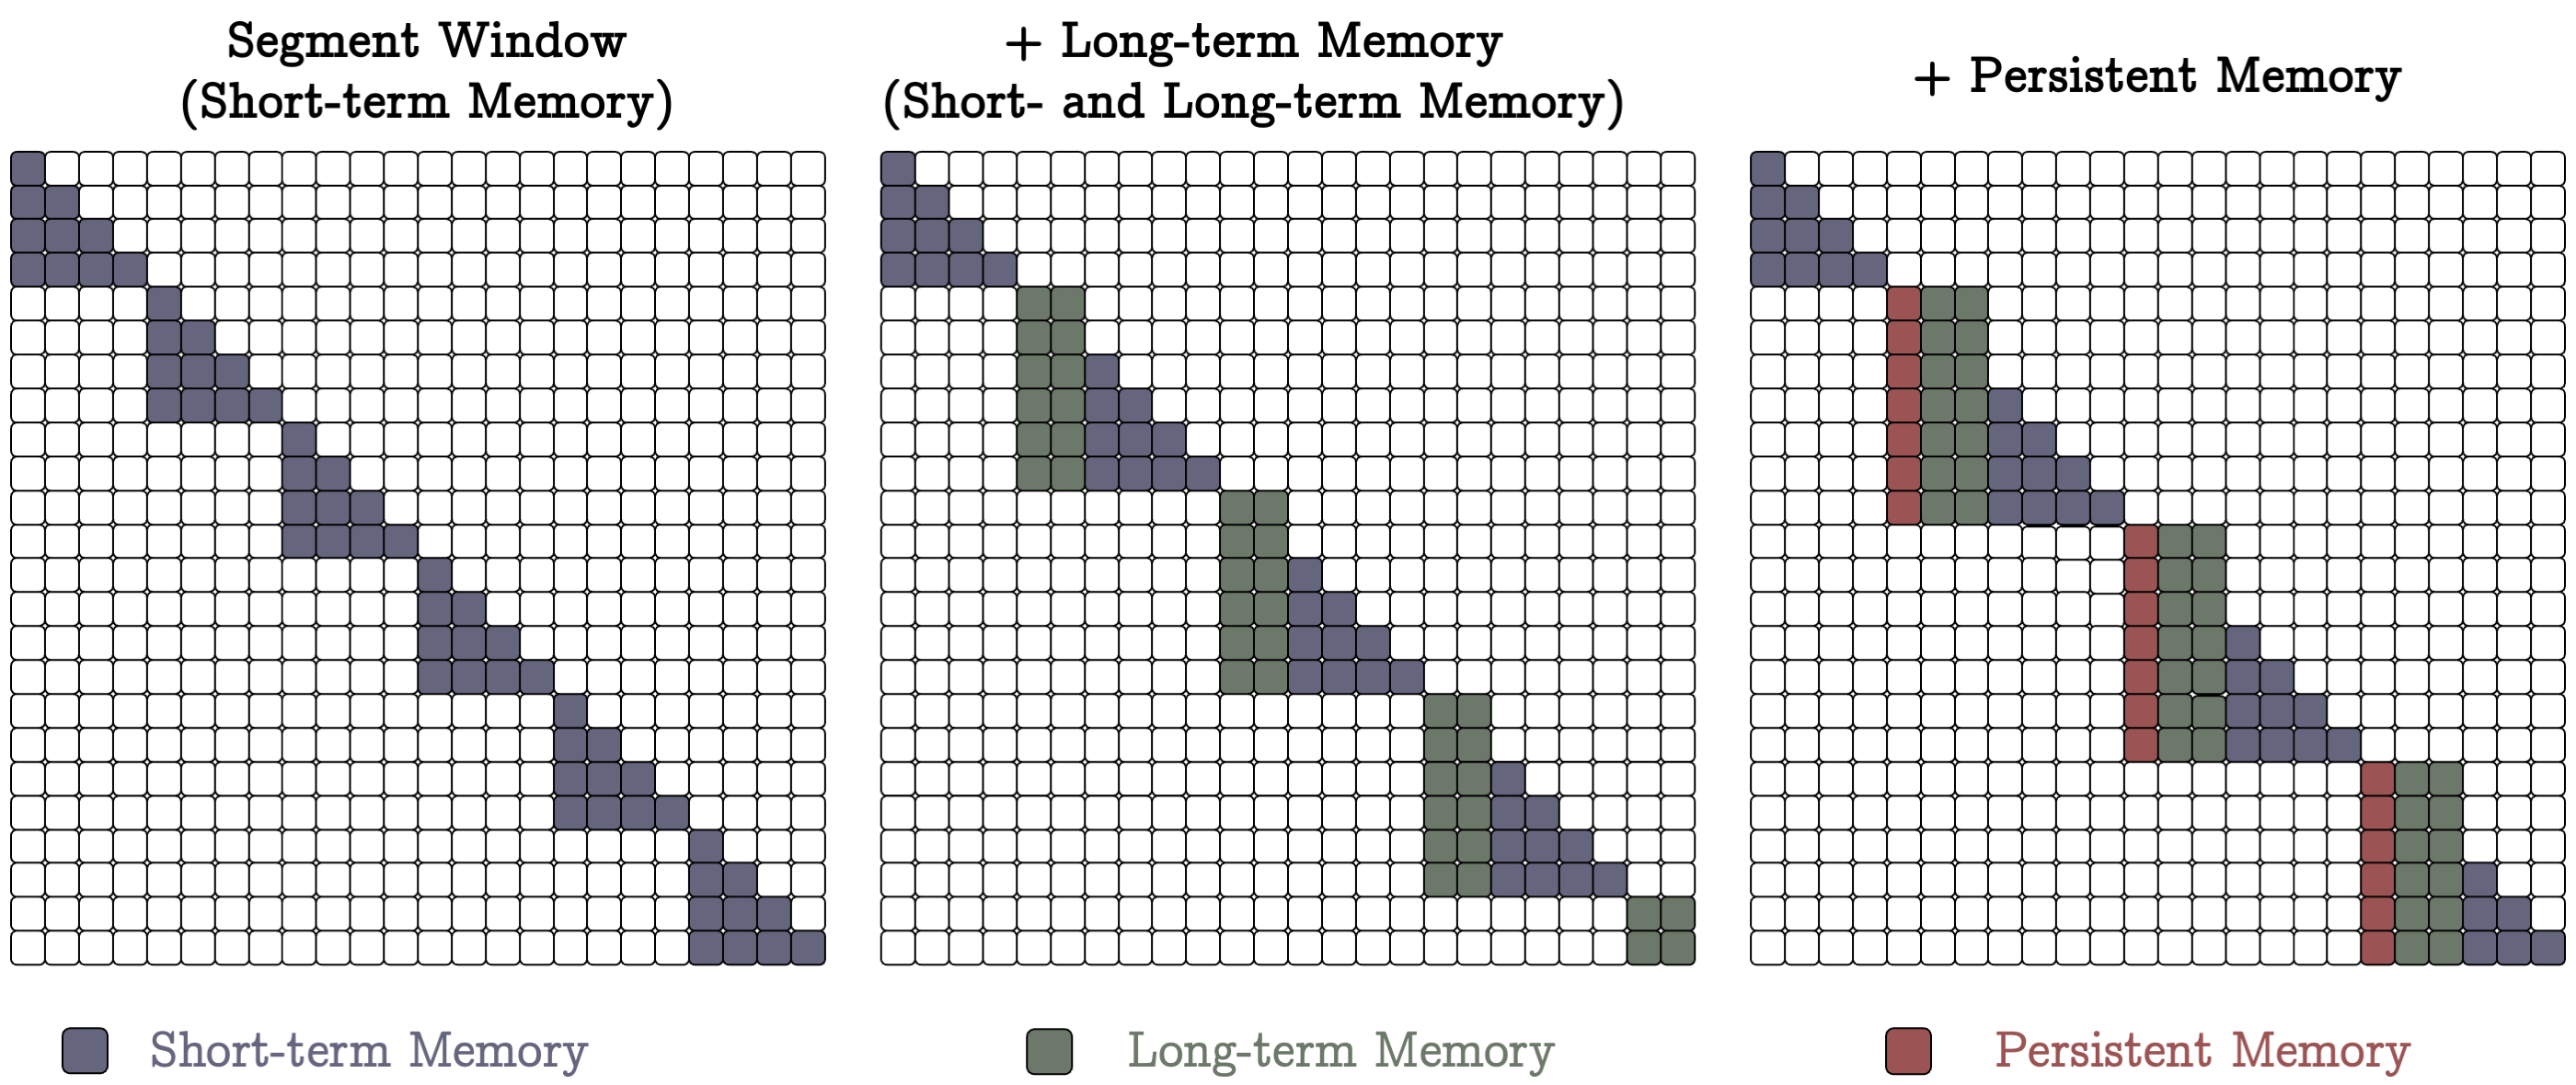
\includegraphics[width=\linewidth]{Figures/MAC.png}
    \caption{\textbf{Memory as a Context (MAC).} We segment the sequence and use full causal attention in each window. Again, the first $N_p$ tokens are persistent memory and the next $N_{l}$ are long-term memory tokens}
    \label{fig:MAC-attention}
    \end{subfigure}~\hfill
    \centering~
    \begin{subfigure}{0.48\linewidth}
        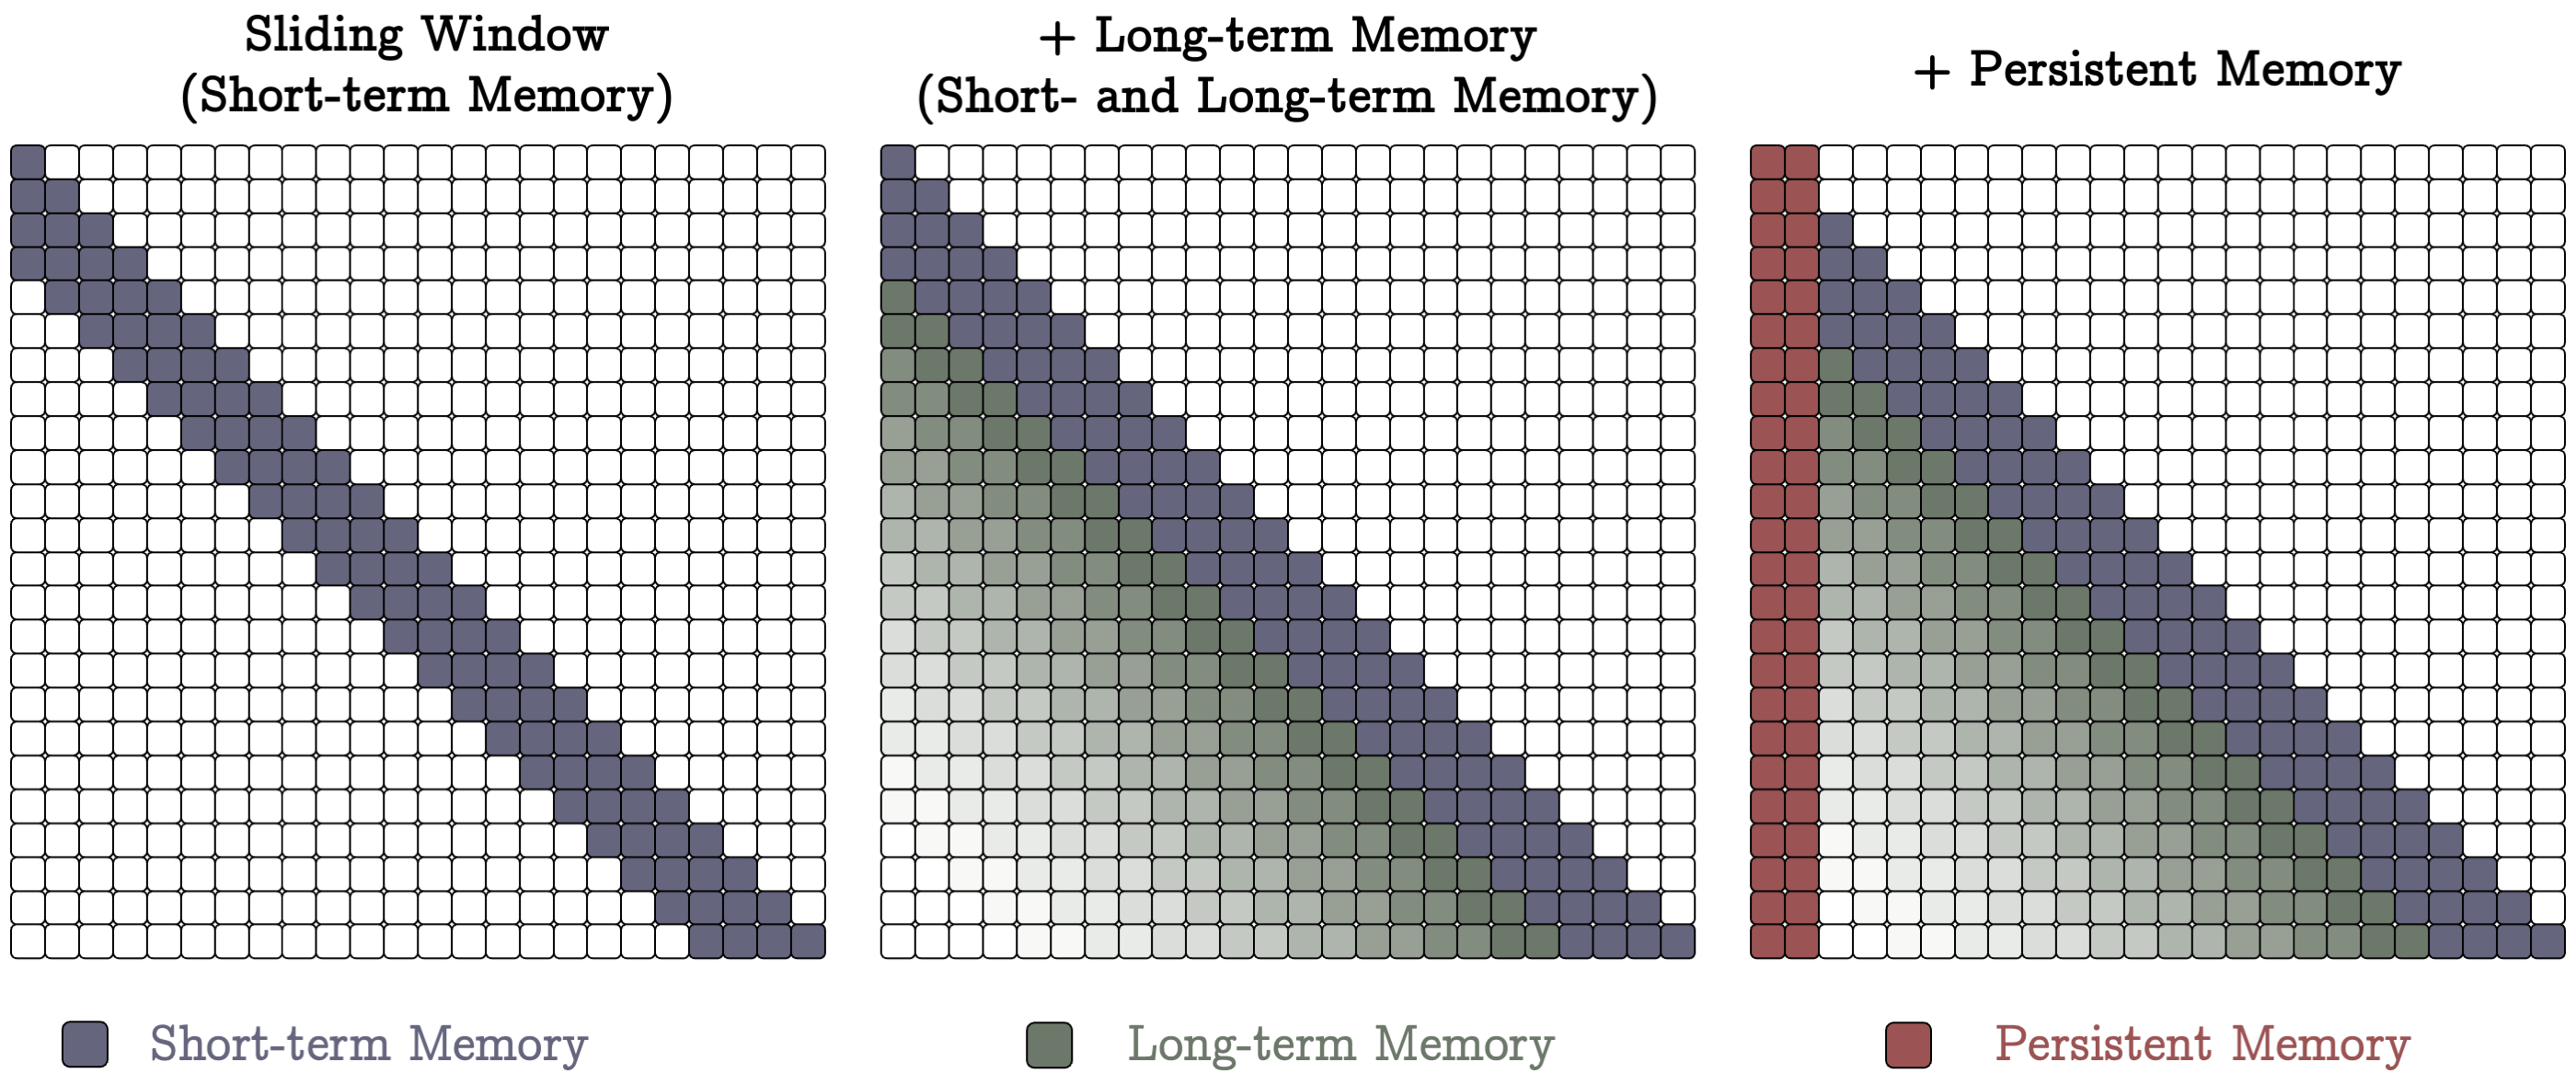
\includegraphics[width=\linewidth]{Figures/MAG.png}
    \caption{\textbf{Memory as Gating (MAG).} We use sliding window attention (SWA) as a short-term memory and our neural memory module as a long-term memory, combining by a gating.}
    \label{fig:MAG-attention}
    \end{subfigure}
    \caption{Attention masks for different variants of Titans.}
\end{figure*}


This architecture has two key advantages: (1) Attention by having both historical and current context, has the ability to decides whether given the current data, the long-term memory information is needed. (2) The attention module helps the long-term memory to store only useful information from the current context. That is, not all tokens in each segment are useful and memorizing all of them can result in memory overflow. Therefore, attention is helping the memory to understand which information is useful, better managing the memory capacity. (3) At test time: (i) persistent memory parameters are fixed as they encodes the knowledge about the task, which should not be changed; (ii) the attention module weights are in-context learner; and (iii) the long-term memory module is still learning (memorizing) the information at test time. That is, we update the weights of the neural memory even at test time as weights are encoding the abstraction of long past.  
















\begin{figure*}[t!]
    \centering
    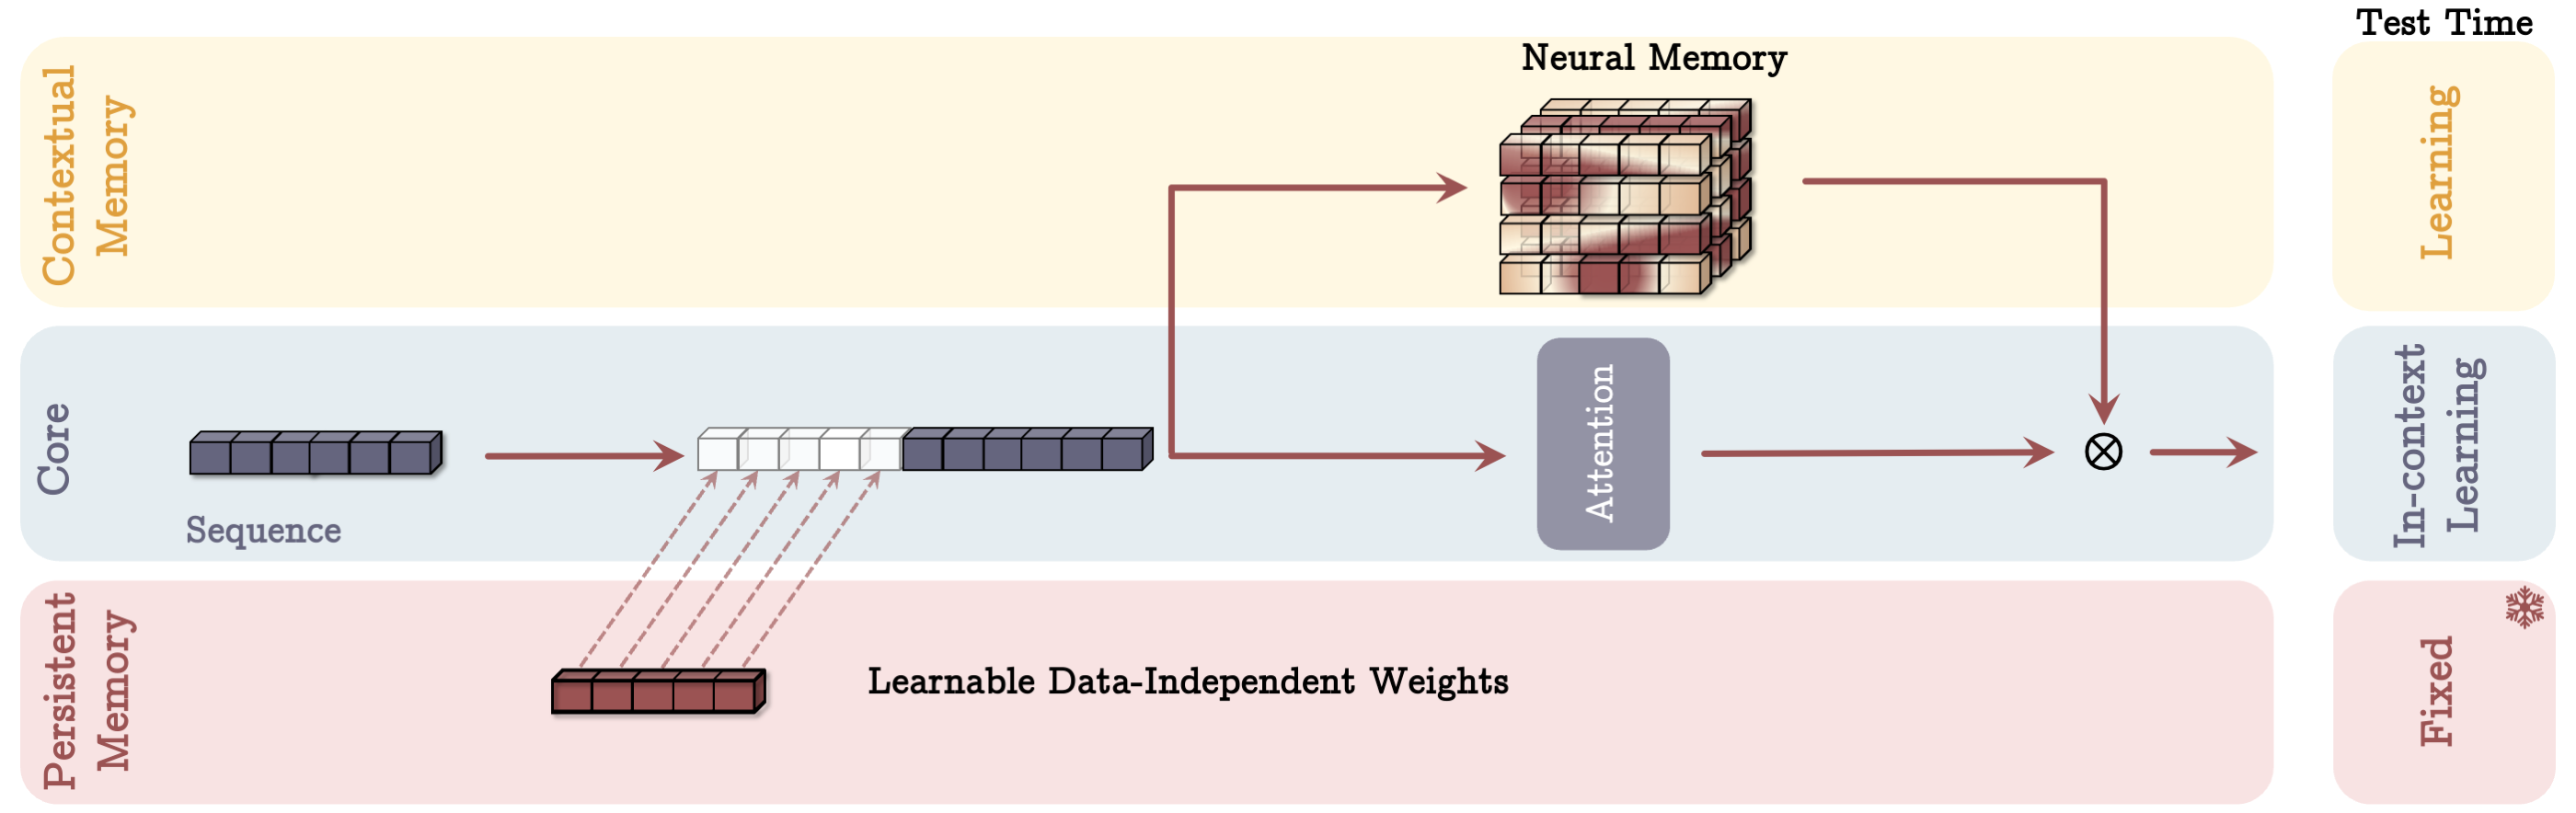
\includegraphics[width=0.9\linewidth]{Figures/gate-arch.png}
    \caption{\textbf{Memory as a Gate (MAG) Architecture.} This architecture, similarly, has the three branches of (1) core, (2) contextual memory, and (3) persistent memory. It, however, incorporates only persistent memory into the context and combine memory with the core branch using a gating mechanism. At test time, the behavior is the same as \autoref{fig:loop-arch}.}
    \label{fig:gate-arch}
\end{figure*}



\subsection{Gated Memory}
In the next variant (see \autoref{fig:gate-arch}), in one branch, we directly use the input data to update the long-term memory, and in the second branch, we use a sliding window attention (SWA):

\begin{align}
    &\tilde{x} = \begin{bmatrix}
    p_1 & p_2 & \dots & p_{N_p}
\end{bmatrix} \:\: || \:\: x, \\
    &y = \texttt{SW-Attn}^*\left( \tilde{x} \right), \\
    &o = y \otimes \M(\tilde{x}),
\end{align}
where $\texttt{SW-Attn}^*$ is sliding window attention with prefix (see \autoref{fig:MAG-attention}). Note that, contrary to the previous design, we are not segmenting the input data. Also, we abuse the notation and use $\M(x)$ to refer to the final output of the memory after all recursion over the tokens of the sequence. In the above equation, $\otimes$ can be any non-linear gating. In our experiments, we normalize the outputs $y$ and $ \M(\tilde{x})$ using learnable vector-valued weights, followed by a non-linearity $\sigma(.)$. 

The overall attention mask of this design is shown in \autoref{fig:MAG-attention}. In this design, sliding window attention is act as a precise short-term memory, while the neural memory module is acting as a fading memory for the model. This architecture design can also be seen as a multi-head architecture where the structure of heads are different~\citep{dong2024hymba}.  








\subsection{Memory as a Layer}
The last variant uses the neural Memory As a Layer (MAL) of a deep neural network (see \autoref{fig:mal}). This architecture design is more common in the literature, where the hybrid models stack recurrent models with full or sliding window attentions. Given input $x$, we have:
\begin{align}
    &\tilde{x} = \begin{bmatrix}
    p_1 & p_2 & \dots & p_{N_p}
\end{bmatrix} \:\: || \:\: x, \\
    &y = \M(\tilde{x}), \\
    &o = \texttt{SW-Attn} \left( y \right),
\end{align}
where $\texttt{SW-Attn}$ is sliding window attention. The main drawback of this design is that the power of the model is limited by each of the layers and so it cannot take advantage of the complementary data processing of attention and neural memory module. In our experiments, for evaluating memory in this design, we use a similar architecture as H3~\citep{fu2023hungry}, where we replace the the sequence model with our neural memory module (LMM).




\begin{figure*}[t!]
    \centering
    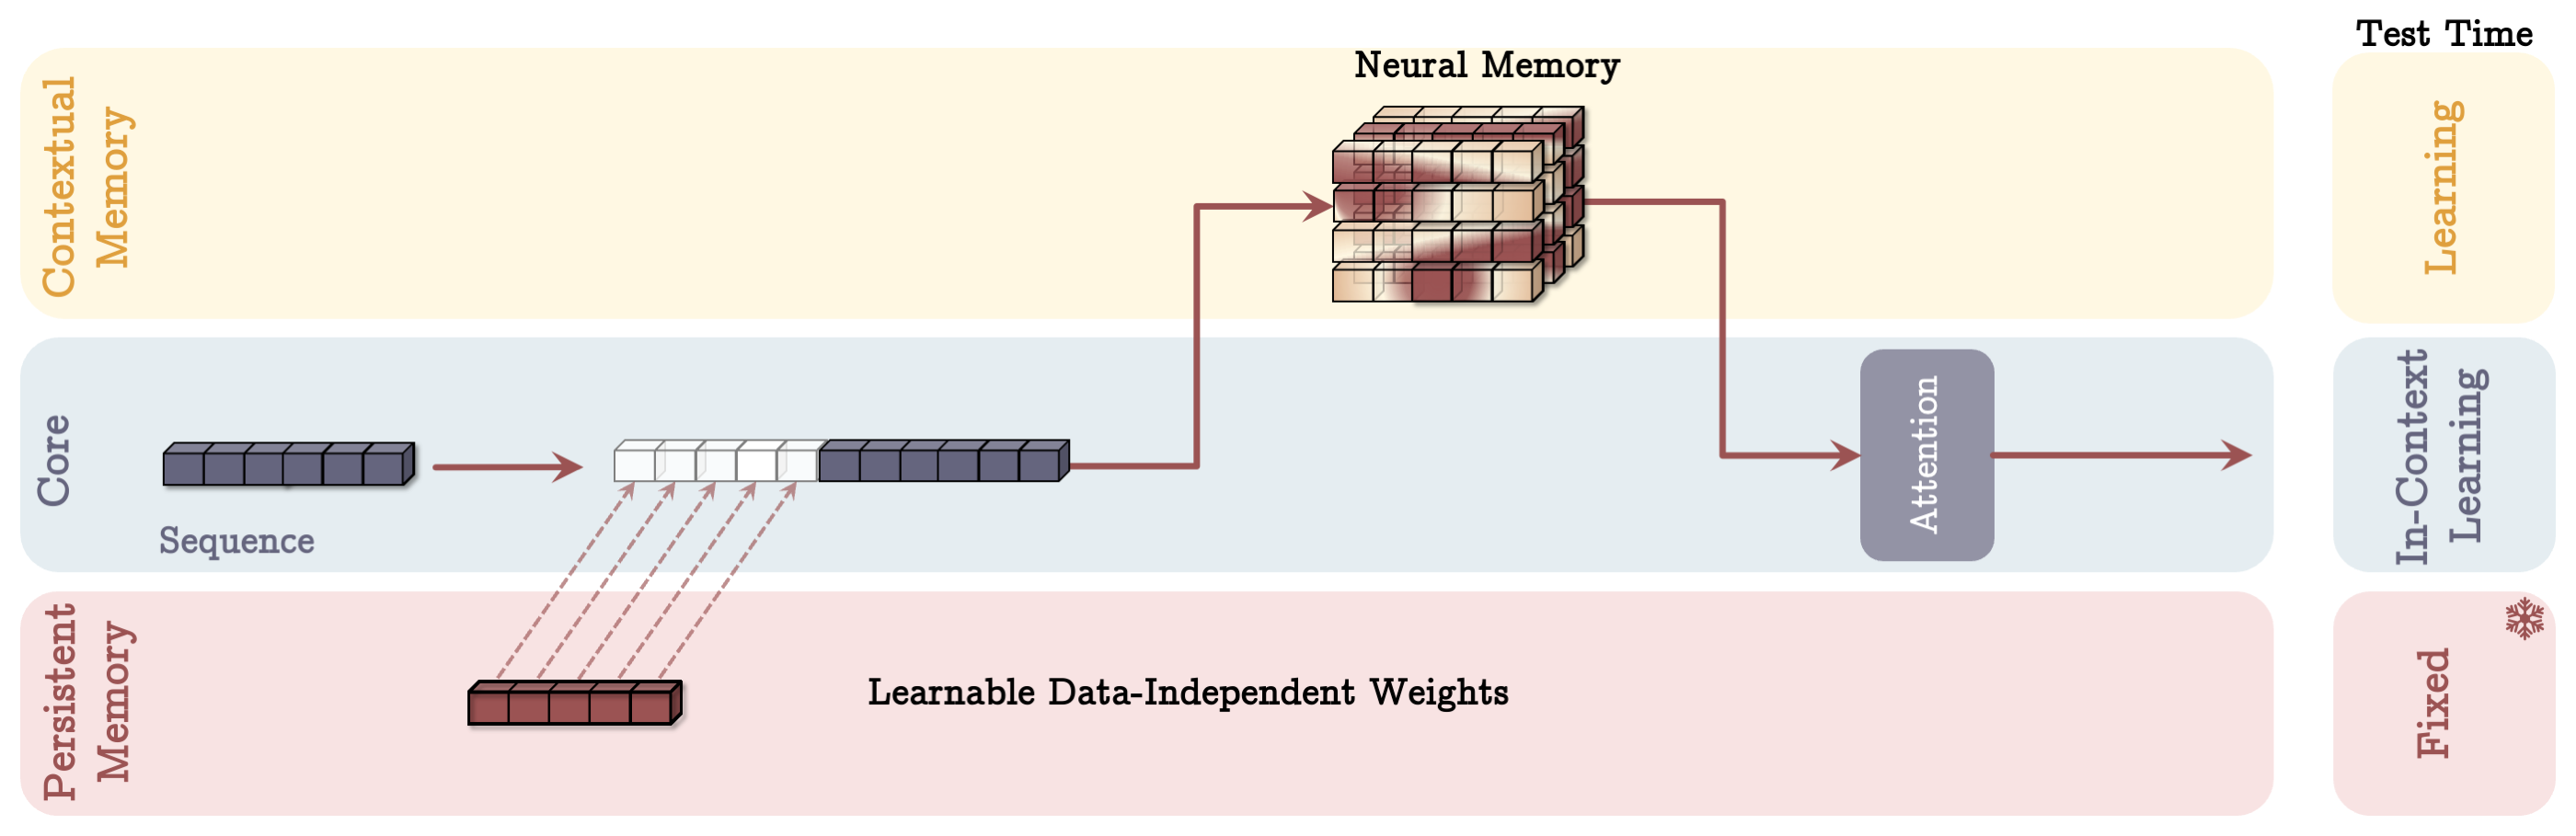
\includegraphics[width=0.9\linewidth]{Figures/MAL.png}
    \caption{\textbf{Memory as a Layer (MAL) Architecture.} In this architecture, the memory layer is responsible to compress the past and current context before the attention module.}
    \label{fig:mal}
\end{figure*}



\head{Memory Without Attention}
Although in the above, we discussed MAL as the combination of LMMs and attention in a sequential manner, one simple variant of MAL is to treat LMM as a sequence model without any attention. From the memory perspective, as discussed in \autoref{sec:intro}, we expect each part of the memory system to work independently, even if other components are disturbed. Therefore, a long-term memory module should still be a powerful model even without short-term memory (i.e., attention). We refer to this variant as LMM or Titans (LMM) in our experiments. We provide additional discussions on the connection of Titans and other modern recurrent models in \autoref{app:MAS}. 



\subsection{Architectural Details}
For the sake of simplicity and presentation, we avoid discussing the implementation details like using residual connection, gating with linear layer, and normalization. In all blocks, we use residual connections. In our implementation, we use \texttt{SiLU}(.) activation~\citep{elfwing2018sigmoid} as the non-linear activation for computing query, key, and values and normalize queries and keys using $\ell_2$-norm. 

\head{Convolution}
Following the recent modern linear recurrent models~\citep{yang2024gated, gu2024mamba}, we  incorporate a 1D depthwise-separable convolution layer after each of the query, key, and value projections. While not significantly affect the performance, these 1D convolutions have shown performance improvement and are also computationally efficient. 


\head{Gating} We also follow the recent architectures that use normalization and gating with a linear layer before the final output projection~\citep{mehta2023long}. 


\begin{theorem}
    Contrary to Transformers, diagonal linear recurrent models, and DeltaNet, all of which are limited to \texttt{TC}$\:^0$~\citep{merrill2024the}, Titans are capable of solving problems beyond \texttt{TC}$\:^0$, meaning that Titans are theoretically more expressive than Transformers and most modern linear recurrent models in state tracking tasks. 
\end{theorem}

